\chapter{Chapter 6: Point Location}

This chapter concerns itself with \textit{point location queries}. Given a map and a query point $q$, in which region is $q$? An application to this is a real-life map. Given a GPS coordinate, which country does the coordinate reside?

\section{Point Location and Trapezoidal Maps}%
\label{subsec:label}

We now formalize this problem a bit. We define the \textit{planar point location problem} as following: Given a \textit{planar subdivision} $\mathcal{S}$ with $n$ edges, how do you store $\mathcal{S}$ in such a way that we can answer queries of the following type: Given a point $q$, report the face, $f$, of $\mathcal{S}$ that contains $q$. If $q$ lies on an edge or coincides with a vertex, the query algorithm should return this information.

\begin{figure}[ht]
	\centering
	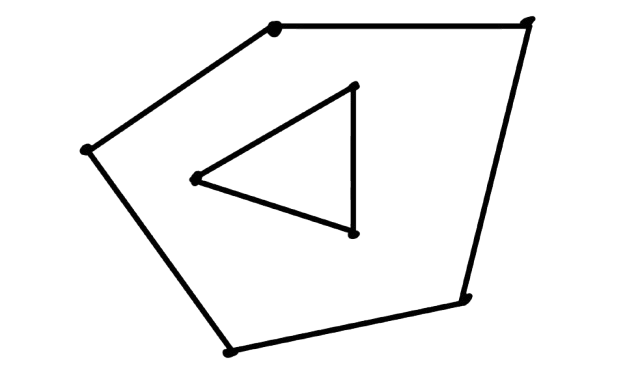
\includegraphics[width=0.5\textwidth]{figures/Map-no-slabs.png}
	\caption{\label{fig:mapnoslabs} A planar subdivision.}
\end{figure}

We now present a very simple data structure to find the face. We draw vertical lines in each of the vertices in the planar subdivision, resulting in what we call \textit{slabs}. We store and sort the $x$-coordinates such that we can find the relevant slab using a binary search tree in $O(\log n)$ time. What is special about a slab, is that there are no vertices inside it. Therefore, all edges intersecting a slab cross it. Because of this, we can order the segments from top to bottom.

\begin{figure}[ht]
	\centering
	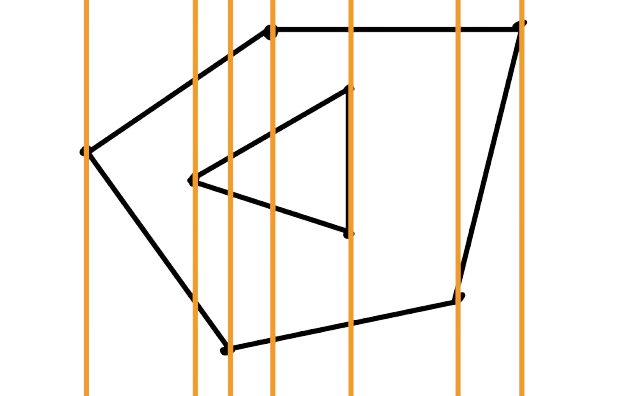
\includegraphics[width=0.5\textwidth]{figures/map-w-slabs.png}
	\caption{\label{fig:mapwithslabs} The subdivision found in~\autoref{fig:mapnoslabs} with slabs.}
\end{figure}


Notice that two segments enclose a face, and the lowest and highest segment are unbounded. Because of this, we can sort these segments in an array. We store along with each segment information about which face it is a part of (i.e., which face is above it). Why we choose the one to be above it, is because this will allow us to find the face easily, when having found the correct slab. We just move downwards, until we find an edge, which then tells us the face. If there is no edge downwards, then we are in the unbounded area.

We now have a bare-bones, but completed, algorithm, which goes like this:

First we do a binary search with the $x$-coordinate for the query point $q$. Then, once we have found the slab, we do a binary search for the $y$-coordinate, giving us the lower segment. This lower segment holds the information about which face we are a part of. If there is no segment below $q$, then $q$ is in the unbounded area.\\
\noindent
\textbf{Query Time}\\
\noindent
The query time for this is good. First we search in the segments, of which there can be at most 2 vertices. As there are $n$ segments, the query time to find the correct slab is $2n$. The second search has at most $n$ vertices (as we have showed earlier), and thus takes $n$ times. Both $2n$ and $n$ can be found using binary search in $O(\log n)$ time.\\
\noindent
\textbf{The Storage Issue}\\
\noindent
We store two arrays: One for the slabs, and one for the $x$-coordinates of the vertices. Since both use $O(n)$ storage, and the array storing the slabs may contain $n$ segments, we may have to store $O(n^{2})$ segments.

In order to solve this issue, we shall introduce the \textit{trapezoidal map}, which is a refinement of $\mathcal{S}$. We say that two line segments in the plane are \textit{non-crossing} if their intersection is either empty or a common endpoints. It is the case for all planar subdivisions that their segments are non-crossing. We will define trapezoidal maps with $S$ being a set of $n$ non-crossing segments in the planes. However, we will also make two simplifications, to make the rest easier for us.
\begin{enumerate}
	\item Surrounding the plane segments is an axis-parallel rectangle $G$. As everything outside $R$ is unbounded, we shall have no problem with this.
	\item No two distinct endpoints of the same segment may share an $x$-coordinate. This is much more unrealistic as these happen in real life.
\end{enumerate}

\begin{figure}[ht]
	\centering
	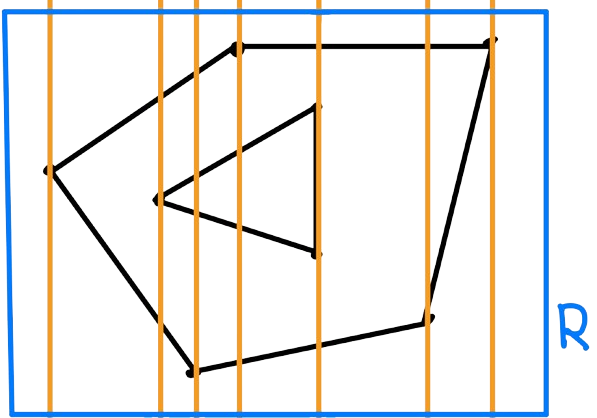
\includegraphics[width=0.5\textwidth]{figures/plane-with-r.png}
	\caption{\label{fig:planewithr} A subdivision with axis-parallel box $R$ surrounding it.}
\end{figure}


We call what we have just defined \textit{a set of line segments in general position}. The \textit{trapezoidal map} which we denote by $\mathcal{T}(S)$ of $S$ is obtained by drawing two vertical extensions from every endpoint $p$ of a segment in $S$, one extension going upwards and one going downwards, until they meet another edge, at which point it stops. We also call this the \textit{vertical decomposition} or \textit{trapezoidal decomposition} of $S$. As we have defined $R$ to be a boundary outside of $S$, the vertical extensions may stop when they reach $R$.

\begin{figure}[ht]
	\centering
	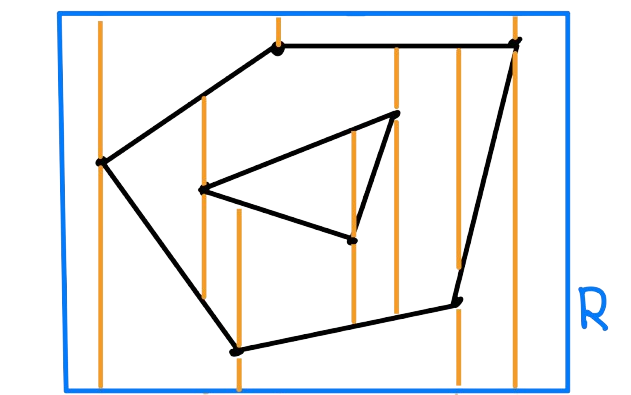
\includegraphics[width=0.5\textwidth]{figures/trapezoidal-map.png}
	\caption{\label{fig:trapezoidalmap} A trapezoidal map.}
\end{figure}

In~\autoref{fig:trapezoidalmap} you can see a trapezoidal map. Notice how this is \textit{almost} the same as the ones in Figures~\ref{fig:mapnoslabs},~\ref{fig:mapwithslabs},~\ref{fig:planewithr}, but it no longer has the problem of one segment having two distinct endpoints with same $x$-value. Furthermore~\ref{fig:trapezoidalmap} has the property of the vertices extending only to the nearest segment. We call the extension going downward the \textit{lower veritcal extension}, and the extension going upward the \textit{upper vertical extension}.

\begin{lemma}
	Each face in a trapezoidal map of a set $S$ of line segments in general position has one or two vertical sides and exactly two non-vertical sides.
\end{lemma}

\begin{proof}
	Let $f$ be a face in $\mathcal{T}(S)$. We must first prove $f$ to be convex.

	One of the requirements for $\mathcal{T}(S)$ was that the segments must be non-crossing. Because of this, any corner of $f$ is either:
	\begin{itemize}
		\item An endpoint of a segment in $S$
		\item A point where a vertical extension abuts a segment of $S$ or an edge of $R$
		\item Or it is a corner of $R$
	\end{itemize}
	Due to the vertical extensions, no corner that is a segment endpoint can have an interior angle great than $180^{\circ}$.

	Because we are looking at the sides of $f$, rather than edges of $\mathcal{T}(S)$ on the boundary of $f$, the convexity of $f$ implies that it can have at most two vertical sides. If we assume $f$ to have more than two sides, we can see that there must be an adjacent vertex which would create a new line, thus restricting the face to a smaller area, with two sides.
\end{proof}

We denote the non-vertical segment of $S$ or edge of $R$ bounding the trapezoid \(\Delta\) from above with $top(\Delta)$ and from below by $bottom(\Delta)$. We can distinguish between five different cases for the left side and right side of a trapezoid \(\Delta\). The cases for the \textit{left side} are as follows:
\begin{enumerate}
	\item It degenerates to a point, which is the common left endpoint of $top(\Delta)$ and $bottom(\Delta)$ (i.e. this forms a triangle).
	\item It is the lower vertical extension of the left endpoint of $top(\Delta)$ that leans on $bottom(\Delta)$.
	\item It is the upper vertical extension of the left endpoint of $bottom(\Delta)$ that lean on $top(\Delta)$
	\item \label{deltap4}It consists of the upper and lower extension of the rig endpoint $p$ of a third segment $s$. These extensions touch on $top(\Delta)$ and $bottom(\Delta)$, respectively.
	\item It is the left edge of $R$. This case occurs only for a single trapezoid of $\mathcal{T}(S)$, namely the unique leftmost trapezoid of $\mathcal{T}(S)$.
\end{enumerate}

The right cases are symmetrical.

We will denote the endpoint defining the left edge of \(\Delta\) by $leftp(\Delta)$. That is, $leftp(\Delta)$ is the left endpoint of $top(\Delta)$ or $bottom(\Delta)$, or in the case of~\autoref{deltap4} it is the right endpoint of a third segment. For the unique \(\Delta\) whose leftside is $R$, we define $leftp(\Delta)$ to be the lower vertex in the vertical segment in $R$. We denote by $rightp(\Delta)$ symmetrically the same as $leftp(\Delta)$.

\begin{lemma}
	The \textit{trapezoidal map} $\mathcal{T}(S)$ of a set $S$ of $n$ line segments in general position contains at most $6n+4$ vertices and at most $3n+1$ trapezoids.
\end{lemma}

\begin{proof}
	A vertex of $\mathcal{T}(S)$ is either a vertex of $R$ or an endpoint of a segment $S$, or the point where another points vertical extension ends. Since every endpoint of a segment induces two vertical extensions, the total number is bounded by $4 + 2n + 2(2n) = 6n+4$. We can find the bound on the total number of trapezoids using Euler's formula. However, we give the direct proof. Recall that each trapezoid has a point $leftp(\Delta)$. By looking at the five cases for the left side, we find that the lower left corner of $R$ plays this role for exactly one trapezoid, a right endpoint of a segment can play this role for at most one trapezoid, and a left endpoint of a segment can be $leftp(\Delta)$ for at most two different trapezoids. It follows that the total number of trapezoids is at most $3n+1$.
\end{proof}


We store trapezoids in such a way that the record for a trapezoid stores pointers to $top(\Delta)$, $bottom(\Delta)$, $leftp(\Delta)$ and $rightp(\Delta)$, and finally the pointers to its at most four neighbours.

\section{A Randomized Incremental Algorithm}%
\label{sec:label}

We want to create an incremental algorithm which constructs the trapezoidal map \textit{and} builds a data structure that can be used to perform point location queries. This is why we don't use the plane sweep algorithm, which would be able to construct the map, but not create the data structure.



%%% Local Variables:
%%% mode: latex
%%% TeX-engine: luatex
%%% TeX-command-extra-options: "-shell-escape"
%%% TeX-master: "main"
%%% End:
